%In this section we explain how to create a solver using \posl{} through an example. \posl{} creates solvers based on local search meta-heuristics algorithms. These algorithms have a common structure: \begin{inparaenum}[1.] \item They start by initializing some data structures (e.g., a \emph{tabu list} for \emph{Tabu Search}~\cite{Gendreau2010}, a \emph{temperature} for \emph{Simulated Annealing}~\cite{Nikolaev2010}, etc.). \item An initial configuration $s$ is generated. \item A new configuration $s'$ is selected from the neighborhood $\mathcal{V}\left(s\right)$. \item If $s'$ is a solution for the problem $P$, then the process stops, and $s'$ is returned. If not, the data structures are updated, and $s'$ is accepted or not for the next iteration, depending on a certain criterion.\end{inparaenum}
%An example of such data structure is the penalizing features of local optima defined by Boussaïd et al~\cite{Boussaid2013} in their algorithm \emph{Guided Local Search}.
%
%%Restarts are classic mechanisms to avoid becoming trapped in local minimum. They are trigged by reaching no improvements or a timeout.
%
%{\it Abstract} \oms{} composing \emph{local search meta--heuristics} are:
%
%\begin{list}{\boxed{Abstract\hspace{4pt}Computation\hspace{4pt}module- \arabic{qcounter}~}}{\usecounter{qcounter}} \itemsep0em 
%	\item $I$: Generating a configuration $s$
%	\item $V$: Defining the neighborhood $\mathcal{V}\left(s\right)$
%	\item $S$: Selecting $s' \in \mathcal{V}\left(s\right)$
%	\item $A$: Evaluating an acceptance criterion for $s'$
%\end{list}
%
%To be more specific in our example, we describe some concrete \oms{} that can be used:
%
%\begin{list}{\boxed{Computation\hspace{4pt}module- \arabic{qcounter}~}}{\usecounter{qcounter}} \itemsep0em 
%	\item $I_{rand}$: Generates a random configuration $s$ \label{estruct:S}
%	\item $V_{1ch}$: Defines the neighborhood $\mathcal{V}\left(s\right)$ changing only one element \label{estruct:V}
%	\item $S_{best}$: Selects the best configuration $s' \in \mathcal{V}\left(s\right)$ improving the current cost. \label{estruct:SS}
%	\item $A_{a.i.}$: Evaluates an acceptance criterion for $s'$. We have chosen the classical module, selecting the configuration with the lowest global cost, {\it i.e.}, the one which is likely the closest to a solution. \label{estruct:A}
%\end{list}

%We can combine modules to create more complex ones. In the example illustrated in this section, I want to apply some selection criteria, but if there is no improvements in the current configuration, a configuration randomly is selected. To do so, we use the operator~$\circled{?}$ to combine the \om{}~\ref{estruct:SS} with another module:
%
%\begin{list}{\boxed{Computation\hspace{4pt}module-3. \arabic{qcounter}~}}{\usecounter{qcounter}} \itemsep0em  
%	\item $S_{rand}$: Selects a random configuration $s' \in \mathcal{V}\left(s\right)$.
%\end{list}

%Let us make consider a slightly more complex solver: When applying the acceptance criteria, suppose that we want to receive a configuration from other solver, to compare it with ours and select the one with the lowest cost. We can do that by applying the operator~$\circled{m}$ to combine the \om{}~\ref{estruct:A} with a \opch:

%\begin{list}{\boxed{Communication\hspace{4pt}module- \arabic{qcounter}:~}}{\usecounter{qcounter}} \itemsep0em
%	\item $C.M.$: Receiving a configuration.\label{struct:opch}
%\end{list}

%Figure~\ref{fig:as_ex} shows a graphic representation of the \as{} that we create for our example. In this Figure all the modules are abstract, so we can instantiate them afterwards to create concrete solvers. Notice that we also want to send the output of the \om{} $A$, in order to share the current configuration with other solvers.
%
%\begin{figure}[h]
%	\centering	
%	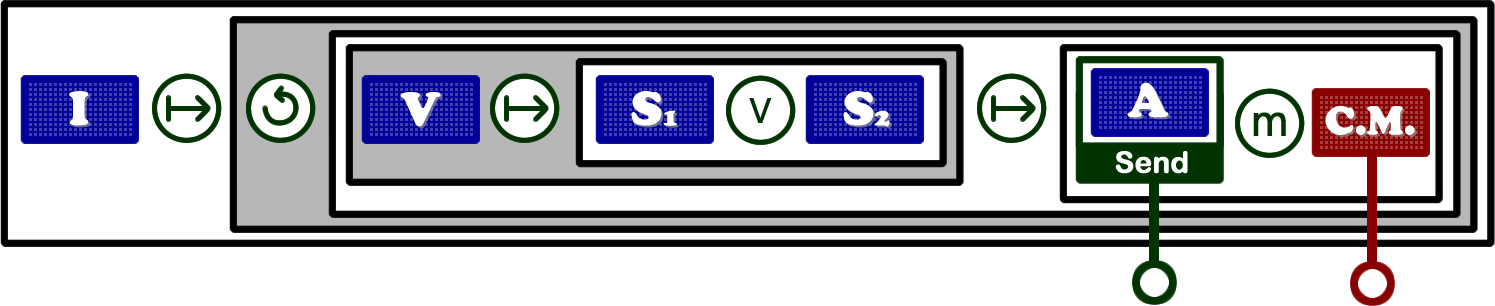
\includegraphics[width=0.7\linewidth]{aexample.png}
%	\caption{Graphic representation of an \as}\label{fig:as_ex}
%\end{figure}
%
%Algorithm \ref{algo:as_ex} shows the \posl{} pseudo-code for the \as{} described above, using predefined operators. Algorithm~\ref{algo:cs_ex} shows the concrete solver definition using the concrete \omprefix{} and \opchs{} already presented. In the later, we have used the concrete \opch{} $CM_{last}$, that receives all the configurations sent to it, and selects the one arriving the last.
%
%In practice, \posl{} provides information regarding the execution process, such as the number of {\sc Iterations}, solver execution {\sc Time}, {\sc Best} found solution, among others.
%
%\begin{algorithm}[H]
%\dontprintsemicolon
%\SetNoline
%\SetKwProg{myproc}{}{}{}
%\myproc{\tet{\bf abstract solver} as\_example\;
%\tet{\bf computation} : $I, V, S_1, S_2, A$ \; 
%\tet{\bf connection}: $C.M.$}{
%	\Begin{
%		%\While{$($\Iter $< K_1)$}
%		%{
%			$I \sec$ \; %\circled{$\mapsto$}$\;
%			\While{$($\Iter \% $K_2)$}{
%				$\left[V \sec \left[S_1\textbf{  } \circled{$\vee$} \textbf{  } S_2\right]\right] \sec \left[\llparenthesis A\rrparenthesis^o \textbf{  } \circled{m} \textbf{  } C.M.\right] $\;
%			}
%		%}
%	}
%}
%\caption{\posl{} pseudo-code for \as{} presented in Figure~\ref{fig:as_ex}}\label{algo:as_ex}
%\end{algorithm}	
%
%\begin{algorithm}[H]
%\dontprintsemicolon
%\SetNoline
%\SetKwProg{myproc}{}{}{}
%%\myproc{
%\tet{\bf solver} S \tet{\bf implements} as\_example\;
%\tet{\bf computation} : $I_{rand}, V_{1ch}, S_{best}, A_{a.i.}$ \; 
%\tet{\bf connection}: $CM_{last}$\; %}{
%%	\Begin{
%%	}
%%}
%\caption{An instantiation of the \as{} in Algorithm~\ref{algo:as_ex}}\label{algo:cs_ex}
%\end{algorithm}

%Now, suppose that I want to create another solver \texttt{Z} using a different neighborhood function, (that we will call $V_{2ch}$) performing two changes instead of only one. As a communication strategy, I also want to connect them through the operator {\it 1~to~N}, using \texttt{Z} as sender and \texttt{S} as receiver. Then,  using namespace expansions,  I need to declare how many solvers we want to connect. Algorithm~\ref{algo:comm_str_ex} shows the desired communication strategy.
%
%\begin{algorithm}[H]
%\dontprintsemicolon
%\SetNoline
%%\myproc{
%[ Z$\cdot A$ (3) ] $\poslop{\rightsquigarrow}$ [ S$\cdot CM_{last}$ (3) ] 2 ;
%\caption{A communication strategy}\label{algo:comm_str_ex}
%\end{algorithm}
%
%\modified{Notice that the connection operation is affected also by the number $2$ at the end of the line, to expand also the topology. In that sense, supposing that we have 12 units of computation available, we obtain a \soset{} working on parallel following the topology described in Figure~\ref{fig:ex_conn}.}
%
%\begin{figure}[h]
%	\centering	
%	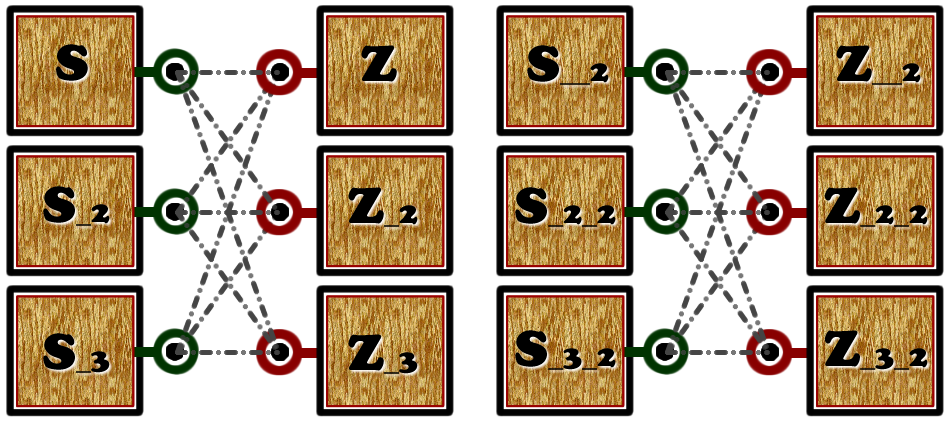
\includegraphics[width=0.6\linewidth]{ex_top.png}
%	\caption{An example of connection strategy for 12 units of computation}\label{fig:ex_conn}
%\end{figure}

%\noindent%
%%\begin{minipage}{\textwidth}
%%	\centering
%\begin{minipage}[t]{.52\textwidth}
%	\begin{algorithm}[H]
%		\caption{Local search meta--heuristic general strategy}
%		\dontprintsemicolon
%		\SetNoline
%		\SetKwProg{myproc}{}{}{}%\mathcal{M}_1^a, \mathcal{M}_1^b,
%		\myproc{$St \leftarrow$ \str \\ \om $: \mathcal{M}_1^a, \mathcal{M}_1^b, \mathcal{M}_2, \mathcal{M}_2, \mathcal{M}_4$ ;\\ \och $: \mathcal{C}h_1$ ;}{
%			\Begin{
%				\While{$($\Iter \% $10000$ $!$= $0)$}{%\mathcal{M}_1^a \circled{$\rho$} \mathcal{M}_1^b
%					$\left[\mathcal{M}_1^a \circled{$\rho$} \mathcal{M}_1^b\right] \longmapsto$\;
%					\While{$($\Iter \% $1000$ $!$= $0)$}{
%						$\left[\mathcal{C}h_1 \circled{$\vee$} \mathcal{M}_2\right] \longmapsto \mathcal{M}_3 \longmapsto \llparenthesis\mathcal{M}_4\rrparenthesis^o$\;
%					}
%				}
%			}
%		}
%		\label{algo:stLSM}
%	\end{algorithm}		
%\end{minipage}
%\hspace{.05\textwidth}
%\begin{minipage}[t]{.40\textwidth}
%	\begin{algorithm}[H]
%		\caption{Local search meta--heuristic solver definition}%
%		\dontprintsemicolon
%		\SetNoline
%		\SetKwProg{myproc}{}{}{}
%		\myproc{$\Sigma_1 \leftarrow$ \solver}{
%			\Begin{%
%				\Strategy{}{St}%
%				%			\oModule{}{$\mathcal{M}_1^a$, $\mathcal{M}_1^b$, $\mathcal{M}_2$, $\mathcal{M}_3$, $\mathcal{M}_4$}
%				\oModule{}{$m_1^a$, $m_1^b$, $m_2$, $m_3$, $m_4$}
%				\oChannel{}{$ch_1$}%
%			}%
%		}%
%		\label{algo:defLSM}%	
%	\end{algorithm}
%\end{minipage}
%%\captionof{figure}{Concrete strategies for Algorithm \ref{algo:mySA}}
%%\label{fig:strategies_sa}
%%\end{minipage}
%\vspace{0.3cm}
%
%Algorithm \ref{algo:defLSM} shows the solver definition. We place here the \cstr{}, followed by instances of the \m s (\module s and \opch s). The instances have to respect the type of the \m s declared in the \cstr.
%%Before declare which are the modules in the solver, it is necessary to instantiate them.
%
%\begin{algorithm} %[H]
%\dontprintsemicolon
%\SetNoline
%%\incmargin{1em}
%$\Sigma_2\cdot\mathcal{M}_{\mathcal{V}} \rightsquigarrow \Sigma_1\cdot\mathcal{C}h_1$
%\caption{Inter--solvers communication definition}%
%\label{algo:defCOMM}%
%\end{algorithm}
%
%Supposing that there exist another solver $\Sigma_2$ with an \module{} called $\mathcal{M}_{\mathcal{V}}$ sharing its neighborhood function, we can connect it with the solver $\Sigma_1$ as the Algorithm \ref{algo:defCOMM} shows.